\documentclass[../main/main.tex]{subfiles}
\begin{document}

\chapter{Instruments d'optique}
\vspace*{-47pt}
\begin{center}
    \Huge Exercices d'application
\end{center}
\section{Tracés de rayons avec association de lentilles}
Les associations de lentilles ne présentent pas de difficultés particulières,
une fois les techniques de construction maîtrisées (cf. chapitre \ref{ch:O1}).

\subsection{}
Dans ce premier cas, on doit construire l'image d'un objet \underline{réel} par
l'association de deux lentilles convergentes. Il suffit pour cela de construire
l'image de l'objet initial $\ABb$ par la lentille $L_1$, image que l'on appellera
$\ABa$. C'est cette image qui servira d'objet à la lentille $L_2$, qui en
formera l'image finale $\ABp$. Pour traduire ce fonctionnement physique, on
notera : $\DS \ABb \underset{O_1}{\overset{\Lc_1}{\longrightarrow}} \ABa
\underset{O_2}{\overset{\Lc_2}{\longrightarrow}}\ABp$ \bigbreak

On procède donc de la même manière que précédemment, en traçant :
\begin{enumerate}
    \item Le rayon passant par $B$ et par $O_1$ : il ne sera pas dévié ;
    \item Le rayon passant par $B$ et par $F_1$ : il émerge parallèle à
        l'A.O. (optionel quand on est sûr-e de ne pas se
        tromper avec les deux autres rayons) ;
    \item Le rayon passant par $B$ et parallèle à l'A.O. : il passe par $F'_1$
        en sortie.
\end{enumerate}

On obtient un faisceau \underline{convergent} en sortie de cette lentille,
l'intersection des rayons se faisant donc dans leur prolongement dans le sens
positif. $\ABa$ est une \underline{image réelle} \underline{\underline{pour
$L_1$}}. \bigbreak

En revanche, cette image, qui est donc l'objet de la lentille $L_2$, est dans
l'espace image de celle-ci : c'est donc un \underline{objet virtuel}
\underline{\underline{pour $L_2$}}. On construit donc son image en trançant :

\begin{enumerate}
    \item Le rayon passant par $B_1$ et par $O_2$ : il ne sera pas dévié ;
    \item Le rayon passant par $B_1$ et par $F_2$ : il émerge parallèle à l'A.O.
        (optionnel) ;
    \item Le rayon passant par $B_1$ et parallèle à l'A.O. : il passe par $F'_2$
        en sortie.
\end{enumerate}

On fait partir les rayons de la gauche du système comme s'ils allaient passer
par $B_1$, mais une fois arrivés à la lentille on continue les traits en
pointillés pour montrer que ce sont des rayons virtuels. Les rayons émergents
suivent les règles de la définition \ref{rconst}, et donnent un faisceau
émergent \underline{convergent} donnant lieu à une \underline{image réelle}.

\begin{center}
    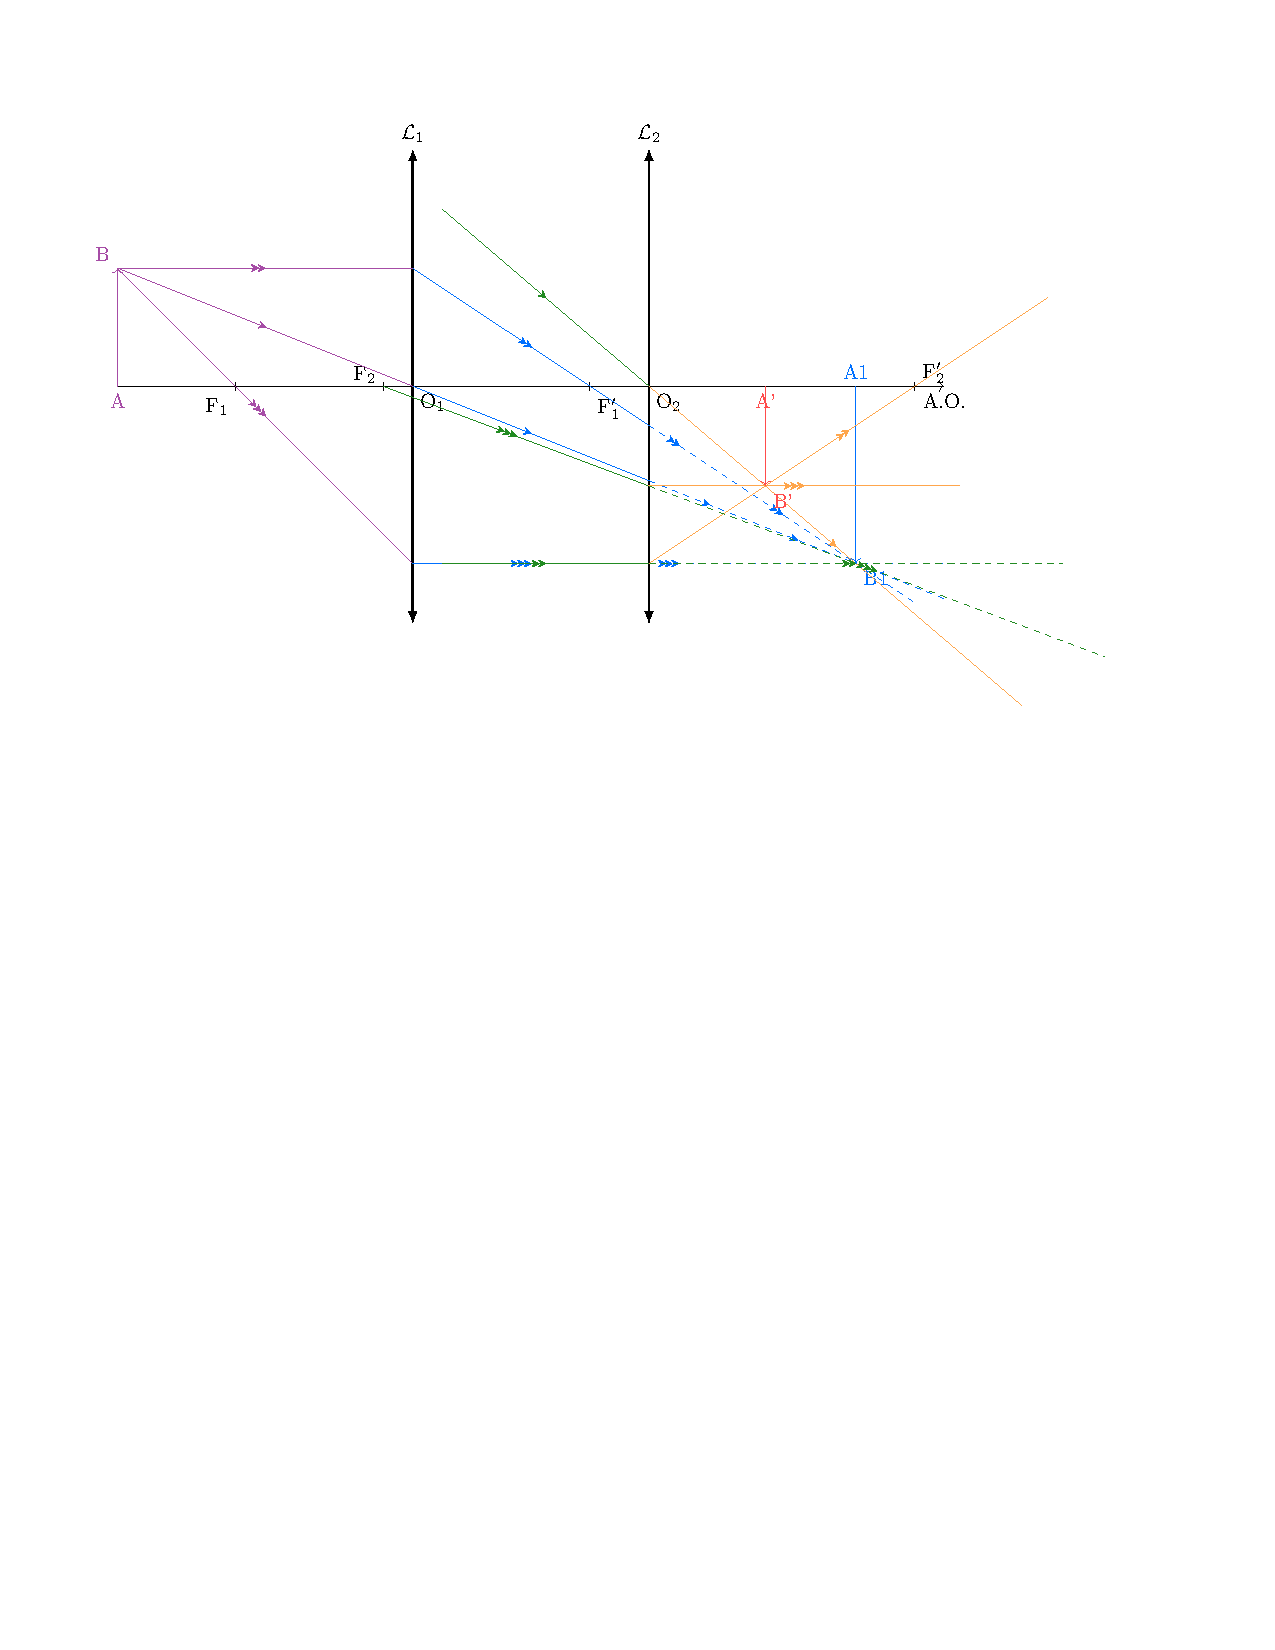
\includegraphics{ch3-1-1}
\end{center}

\subsection{}
De la même manière, on construit $\ABa$ à partir de l'action de $L_1$ sur
$\ABb$.  C'est la situation 1) 1- c. pour la lentille convergente : on obtient
une \underline{image virtuelle} \underline{\underline{pour $L_1$}}. $\ABa$ est
cependant dans l'espace objet pour $L_2$, et est donc un \underline{objet réel}
\underline{\underline{pour $L_2$}}. On construit son image comme dans la
situation 1) 1- a. pour la lentille divergente, et on obtient une
\underline{image virtuelle}.

\begin{center}
    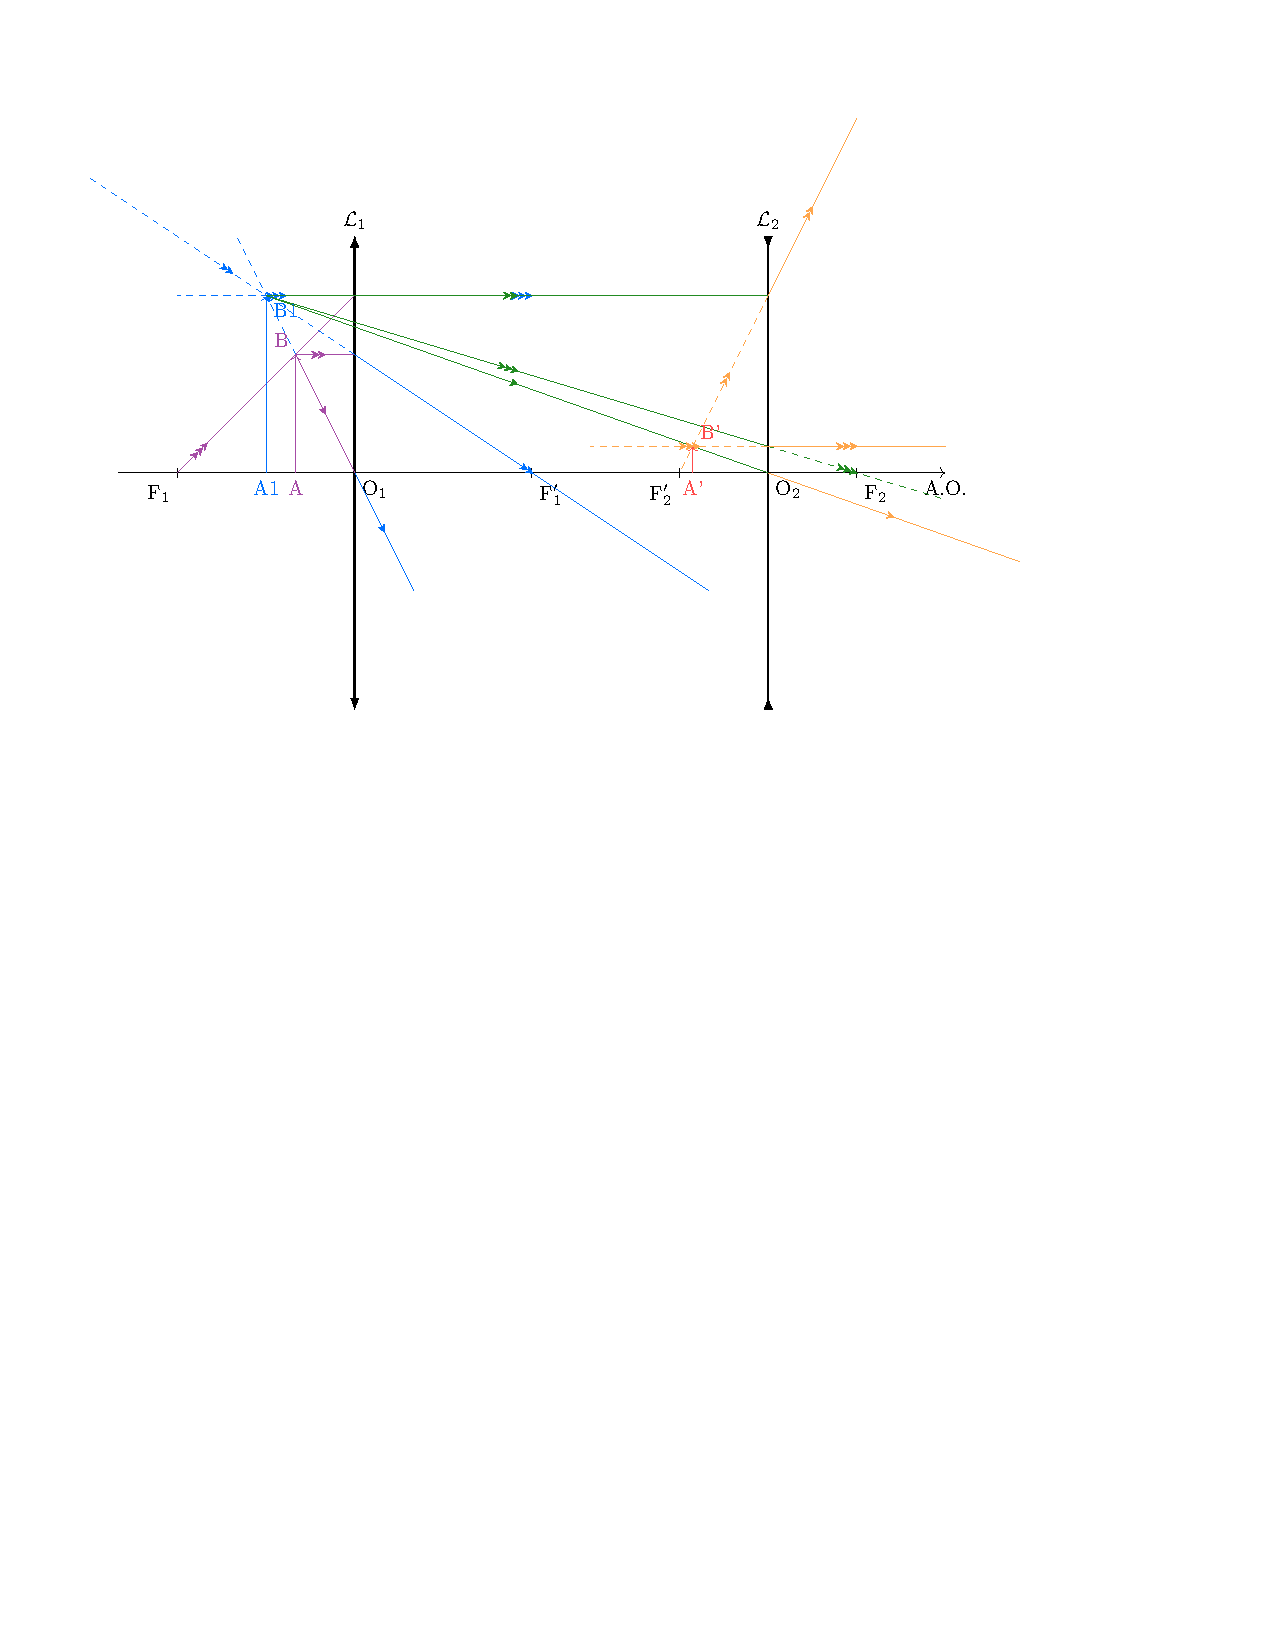
\includegraphics{ch3-1-2}
\end{center}

\section{Des lunettes astronomiques}
\begin{center}
    \huge Partie 1
\end{center}

\begin{center}
    \begin{NCdefi}[width=.7\linewidth]{Données}
    Association de deux lentilles :
    \begin{enumerate}
        \item $L_1$ « objectif », vergence $C_1 = \SI{3.125}{\de}$, diamètre $D
            = \SI{30}{mm}$ ;
        \item $L_2$ « oculaire », vergence $C_2 = \SI{25}{\de}$.
    \end{enumerate}
\end{NCdefi}
\end{center}

\subsection{}

\begin{tcbraster}[raster columns=3, raster equal height=rows]
    \begin{NCprop}{Résultat attendu}
        Focales de lentilles
    \end{NCprop}
    \begin{NCdemo}{Outil du cours}
        Une lentille de focale $f'$ a pour vergence $V$ :
        \[ V = \frac{1}{f'} \]
    \end{NCdemo}
    \begin{NCexem}{Application}
        \[ \boxed{\obar{O_1F'_1} = \SI{32}{cm}} \]
        \[ \boxed{\obar{O_2F'_2} = \SI{4}{cm}} \]
    \end{NCexem}
\end{tcbraster}

\subsection{a.}
\begin{tcbraster}[raster columns=2, raster equal height=rows]
    \begin{defi}{Système afocal}
        Est afocal un système pour lequel un objet initial à l'infini donne une
        image finale à l'infini.
    \end{defi}
    \begin{inte}{Intérêt d'un système afocal}
        Un système afocal présente comme intérêt de permettre à un œil emmétrope
        d'observer sans fatigue, étant donné que l'image sortant du système est à
        l'infini (cf chapitre 1 exercice 4).
    \end{inte}
\end{tcbraster}

\setcounter{subsection}{1}
\subsection{b.}

\begin{tcbraster}[raster columns=6, raster equal height=rows]
    \begin{NCprop}[raster multicolumn=1]{Résultat attendu}
        $$\obar{O_1O_2}$$
    \end{NCprop}
    \begin{NCdemo}[raster multicolumn=2]{Outils du cours}
        Règles de construction de rayons :
        \begin{enumerate}
            \item Un rayon provenant de l'infini émerge d'une lentille en croisant
                l'axe optique au plan focal image ;
            \item Des rayons se croisant dans le plan focal objet d'une lentille
                émergent parallèles entre eux.
        \end{enumerate}
        Relation de Chasles :
        \[ \obar{O_1O_2} = \obar{O_1F_1'} + \obar{F_1'O_2} \]
    \end{NCdemo}
    \begin{NCexem}[raster multicolumn=3]{Application}
        Pour que tous les rayons sortant de la lunette soient parallèles entre eux
        (donnant donc une image à l'infini), il faut que tous les rayons à
        l'intérieur passent par le plan focal objet de son oculaire.\bigbreak
        Or, tous les rayons arrivent dans la lunette parallèles entre eux (objet
        initial à l'infini) ; il se croisent donc dans le plan focal image de
        l'objectif. \bigbreak
        Pour que la condition soit vérifiée, il faut donc simplement que les plans
        focaux image de $L_1$ et objet de $L_2$ soient confondus ; autrement dit :
        \[ \boxed{F_1' = F_2} \]
        On a alors $\obar{O_1O_2} = \obar{O_1F_1'} + \obar{F_2O_2}$, et finalement
        \[ \boxed{\obar{O_1O_2} = \SI{+36}{cm}} \]
    \end{NCexem}
\end{tcbraster}

\setcounter{subsection}{1}
\subsection{c.}
Pour cette question, le placement de l'image intermédiaire ne nécessite que le
tracé du rayon passant par $O_1$, étant donné que son intersection avec le plan
focal image donnera la position de $B_1$ :

\begin{center}
    \begin{NCrapp}[width=.7\linewidth]{Rappel}
        \begin{itemize}
            \item Deux rayons parallèles avant le système optique se coupent
                dans le plan focal image ;
            \item Deux rayons qui se coupent dans le plan focal objet émergent
                parallèles entre eux.
        \end{itemize}
    \end{NCrapp}
\end{center}

On peut donc facilement tracer les rayons émergents du «~pinceau~» (i.e.
l'espace entre les deux rayons entrant) puisqu'ils doivent se croiser en $B_1$.
Sur le schéma suivant, les rayons sortant sont également tracés, et cette fois
on utilise la seconde partie du rappel précédent : les deux rayons bleus se
coupant en $B_1$ émergent parallèle entre eux, et il suffit de construire un
rayon émergent de $B_1$ (par exemple celui passant par $O_2$ et qui n'est pas
dévié) pour trouver l'angle de sortie.

\begin{center}
    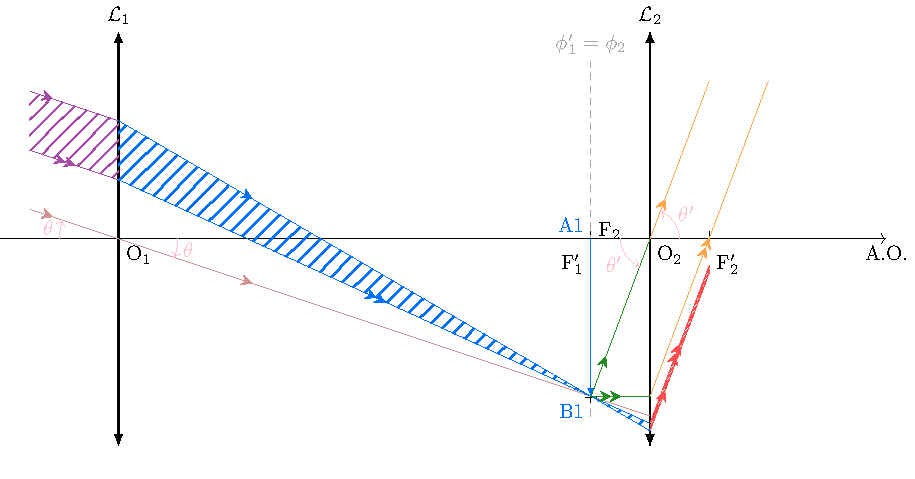
\includegraphics{ch3-2-1_kepler}
\end{center}

\setcounter{subsection}{1}
\subsection{d.}
\begin{tcbraster}[raster columns=6, raster equal height=rows]
    \begin{NCprop}{Résultat attendu}
        Grossissement de la lunette
    \end{NCprop}
    \begin{NCdemo}{Outil}
        \[ G = \frac{\theta'}{\theta}\]
    \end{NCdemo}
    \begin{NCexem}[raster multicolumn=2]{Application}
        Avec le tracé sur le schéma et en considérant des petits angles,
        $\DS \theta' = \frac{\ABa}{\obar{O_2F_2}} > 0$ et $\DS \theta =
        \frac{\ABa}{\obar{O_1F_1'}} < 0$, soit \[ G = \frac{f_1'}{-f_2'} = -8\]
    \end{NCexem}
    \begin{NCimpo}[raster multicolumn=2]{Attention}
        Pour bien voir si un angle est positif ou négatif, il faut se donner un
        sens dans lequel compter positivement, tracer les angles depuis l'axe
        optique jusqu'au rayon pour voir le changement de direction et dans la
        formule trigonométrique utiliser les grandeurs dans le bon sens.
    \end{NCimpo}
\end{tcbraster}

\subsection{a.}
\begin{tcbraster}[raster columns=2, raster equal height=rows]
    \begin{defi}{Cercle oculaire}
        On appelle cercle oculaire l'image de la monture de l'objectif donnée par
        l'oculaire.
    \end{defi}
    \begin{inte}{Utilité du cercle oculaire}
        Il correspond à la section la plus étroite du faisceau sortant de
        l'oculaire, où l'œil reçoit le maximum de lumière.  
    \end{inte}
\end{tcbraster}

\setcounter{subsection}{2}
\subsection{b.}

\begin{tcbraster}[raster columns=6, raster equal height=rows]
    \begin{NCprop}[raster multicolumn=1]{Résultat attendu}
        $$\obar{O_2C_k'}$$
    \end{NCprop}
    \begin{NCdemo}[raster multicolumn=2]{Outil du cours}
        Par définition, $C_k'$ est l'image de $O_1$ par $L_2$. On va donc se servir
        de la relation de conjugaison d'une lentille mince :
        \[ \frac{1}{\OF} = \frac{1}{\OAp} - \frac{1}{\OA} \]
    \end{NCdemo}
    \begin{NCexem}[raster multicolumn=3]{Application}
        On a ici $O \equiv O_2$, $F' \equiv F_2'$, $A \equiv O_1$ et $A' \equiv
        C_k'$. On a donc :
        \[ \frac{1}{\obar{O_2F_2'}} = \frac{1}{\obar{O_2C_k'}} -
        \frac{1}{\obar{O_2O_1}} \]
        et après calculs :
        \[ \boxed{\obar{O_2C_k'} = \left[ \frac{1}{\obar{O_2O_1}} +
        \frac{1}{\obar{O_2F_2'}}\right]^{-1} = \SI{+4.5}{cm}} \]
    \end{NCexem}
\end{tcbraster}

\setcounter{subsection}{2}
\subsection{c.}
\begin{tcbraster}[raster columns=5, raster equal height=rows]
    \begin{NCprop}[raster multicolumn=1]{Résultat attendu}
        $$D_k'$$
    \end{NCprop}
    \begin{NCdemo}[raster multicolumn=2]{Outil du cours}
        Le diamètre du cercle oculaire s'apparente à la taille d'un objet. On peut
        donc utiliser le grandissement :
        \[ \g = \frac{\ABp}{\ABb} = \frac{\OAp}{\OA} \]
    \end{NCdemo}
    \begin{NCexem}[raster multicolumn=2]{Application}
        Avec les données de l'énoncé, on obtient :
        \[ \g = \frac{D_k'}{D} = \frac{\obar{O_2C_k'}}{\obar{O_2O_1}}\]
        et finalement
        \[ \boxed{D_k' = D\times \frac{\obar{O_2C_k'}}{\obar{O_2O_1}} =
        \SI{3.75}{mm}} \]
    \end{NCexem}
    
\end{tcbraster}

\begin{center}
    \huge Partie 2
\end{center}

\subsection{}
Si l'oculaire est divergent, cela signifie que $C_3 < 0$. On a donc $C_3 = -
C_2$, d'où le résultat demandé.

\subsection{}
On reprend la question 2) b-, avec cette fois des indices « 3 » au lieu des
indices « 2 », et on obtient :

\begin{tcbraster}[raster columns=2, raster equal height=rows]
    \begin{NCexem}{Application}
        $\obar{O_1O_3} = \obar{O_1F_1'} + \obar{F_3O_3}$ avec $\obar{F_3O_3} =
        \obar{O_3F_3'} = \SI{-4}{cm}$, d'où
        \[ \boxed{\obar{O_1O_3} = \SI{+28}{cm}} \]
    \end{NCexem}
    \begin{inte}{Intérêt}
        La lunette de Galilée est donc plus compacte que la lunette de Kepler !
    \end{inte}
\end{tcbraster}
\vfill
\subsection{}

\begin{center}
    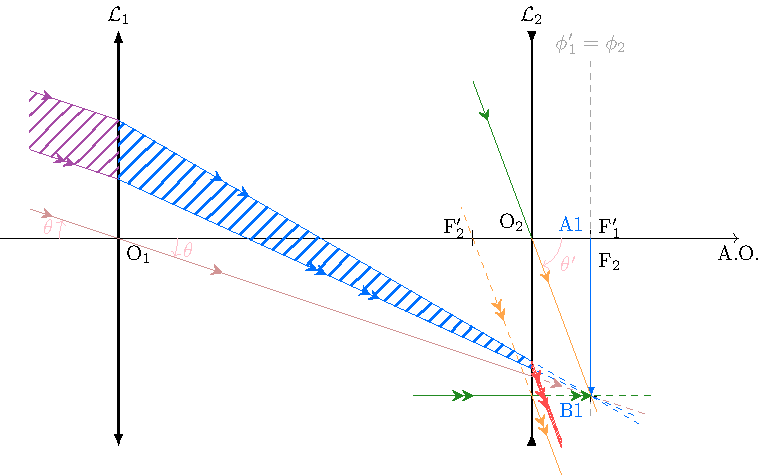
\includegraphics{ch3-2-2_galilee}
\end{center}

\subsection{a.}
On reprend la question 2) 3- b., avec des indices « 3 » au lieu de « 2 », et on
obtient :
\begin{tcbraster}[raster columns=3, raster equal height=rows]
    \begin{NCexem}[raster multicolumn=1]{Application}
        \[ \boxed{\obar{O_3C_k'} = \SI{-3.5}{cm}}\]
    \end{NCexem}
    \begin{NCrema}[raster multicolumn=2]{Comparaison}
        On a cette fois un cercle oculaire virtuel. Il faudra placer son œil le plus
        près possible de l'oculaire pour espérer avoir le plus de lumière possible.
    \end{NCrema}
\end{tcbraster}

\setcounter{subsection}{6}
\subsection{b.}
On reprend la question 2) 3- c. :
\begin{center}
    \begin{NCexem}[width=.3\linewidth]{Application}
        \[ \boxed{D_k' = \SI{3.75}{mm}} \]
    \end{NCexem}
\end{center}

\subsection{Comparaison}
\begin{center}
    \begin{tabularx}{.7\linewidth}{|Y*{2}{|Y}|}\hline
        \rowcolor{gray!15} & Avantages & Inconvénients \\\hline
        \cellcolor{gray!15} Lunette Galilée & + compacte\smallbreak image droite &
        cercle oculaire virtuel \\\hline
        \cellcolor{gray!15} Lunette Kepler & Grande clarté \smallbreak Cercle
        oculaire réel & - compacte \smallbreak image renversée \\\hline
    \end{tabularx}
\end{center}

\vfill

\section{L'œil hypermétrope et sa correction}
\begin{center}
    \begin{NCdefi}[width=.9\linewidth, sidebyside]{Données}
        \begin{itemize}
            \item Œil = lentille $(\Lc, S)$ ;
            \item $\obar{SE} = \SI{17}{mm}$ ;
            \item $\obar{SA} = -\infty \Rightarrow \obar{SA'} = \obar{SE} +
                \SI{1.5}{mm}$
        \end{itemize}
        \tcblower
        \tcbsubtitle[before skip=\baselineskip,
        colback = green!50!black,
        colframe = green!50!black]{Schéma}
        \begin{center}
            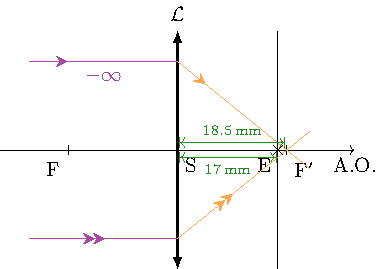
\includegraphics{ch3-3-1}
        \end{center}
    \end{NCdefi}
\end{center}

\subsection{}
\begin{tcbraster}[raster columns=5, raster equal height=rows]
    \begin{NCprop}{Résultat attendu}
        \[\obar{SF'}\]
    \end{NCprop}
    \begin{NCdemo}[raster multicolumn=2]{Outil}
        On trouve le point focal image d'un système en étudiant l'image d'un
        objet à l'infini.
    \end{NCdemo}
    \begin{NCexem}[raster multicolumn=2]{Application}
        Ici, la lecture de l'énoncé donne directement la réponse : le point
        focal image et \SI{1.5}{mm} derrière la rétine. On a donc \[\obar{SF'} =
        \SI{18.5}{mm}\]
    \end{NCexem}
\end{tcbraster}
\subsection{}
L'œil n'est pas assez convergent, il faudrait que les rayons se croisent plus
tôt sur l'axe optique pour que l'image se forme sur la rétine. Il faut donc
corriger avec des lentilles correctrices convergentes.

\subsection{}
\begin{center}
    \begin{NCdefi}[width=.9\linewidth, sidebyside]{Données}
        \begin{itemize}
            \item Verre lunette = $(\Lc_v, O)$ ;
            \item $\obar{OS} = \SI{12}{mm}$ ;
            \item $\ABb \opto{\Lc_v}{O} \ABa \opto{\Lc}{S} \ABp$
        \end{itemize}
        \tcblower
        \tcbsubtitle[before skip=\baselineskip,
        colback = green!50!black,
        colframe = green!50!black]{Schéma}
        \begin{center}
            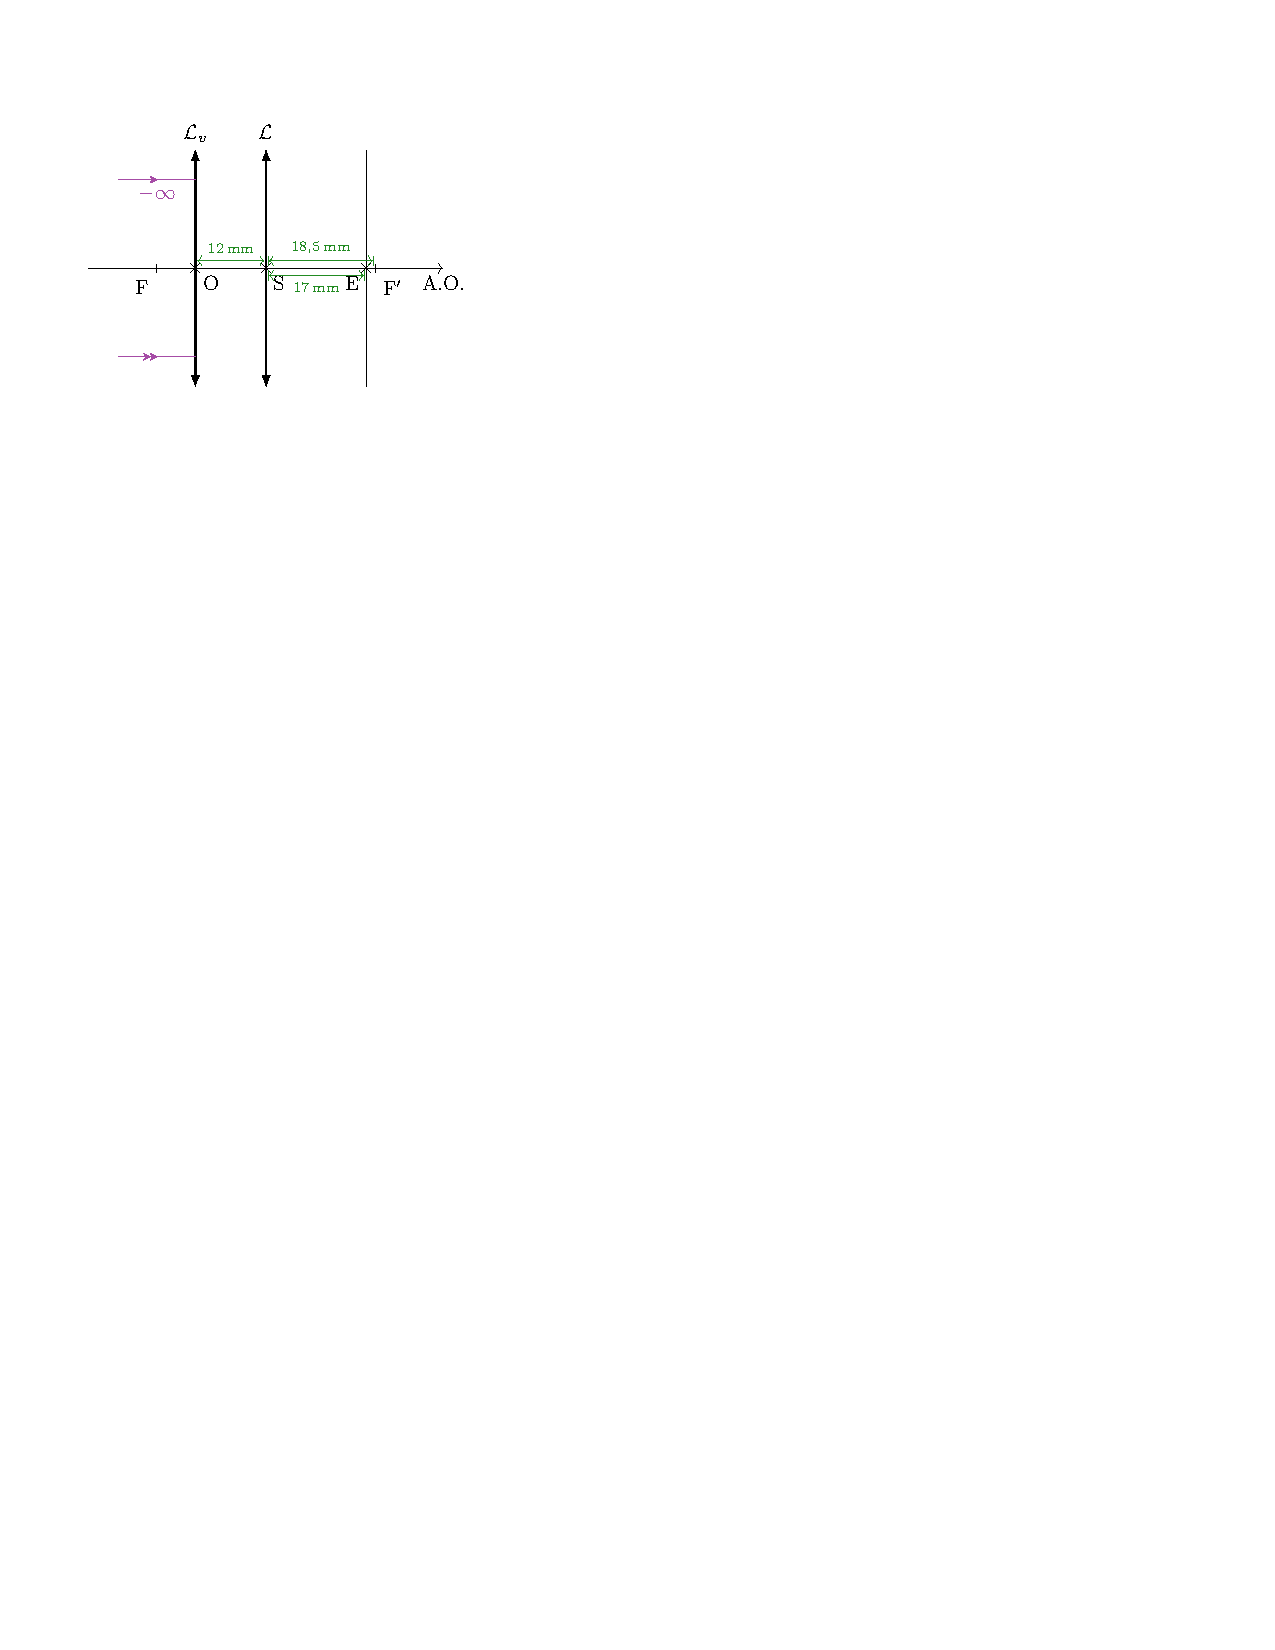
\includegraphics{ch3-3-2}
        \end{center}
    \end{NCdefi}
\end{center}

\subsubsection{}
\begin{center}
    \begin{NCrapp}[width=.5\linewidth]{Rappel}
        L'image doit se former sur l'écran de la lentille, autrement dit la
        rétine : avec $\ABb = -\infty$ on doit avoir $A' = E$.
    \end{NCrapp}
\end{center}

\subsubsection{}
\begin{tcbraster}[raster columns=3, raster equal height=rows]
    \begin{NCprop}{Résultat attendu}
        Utiliser le fonctionnement physique du système pour déterminer comme
        associer la lunette à l'œil.
    \end{NCprop}
    \begin{NCimpo}{Important !}
        Attention, \textbf{seul} le remotum\endnote{\textcolor{black}{remotum} :
        point de l'espace qu'un œil, emmétrope ou non, voit net sans accomoder.
    Pour l'œil hypermétrope, il se situe derrière l'œil.} de l'œil emmétrope est
    à l'infini. Vérifiez bien vos définitions.
    \end{NCimpo}
    \begin{NCexem}{Application}
        \begin{center}
            \begin{tikzpicture}[]
                \node[] (AB) at (0,0) {$\ABb$};
                \node[] (A_1B_1) at (2,0) {$\ABa$};
                \node[] (A'B') at (4,0) {$\ABp$};
                \draw[->] (AB) -- (A_1B_1)
                    node [midway, above] {$\Lc_v$}
                    node [midway, below] {O};
                \draw[->] (A_1B_1) -- (A'B')
                    node [midway, above] {$\Lc$}
                    node [midway, below] {S};
                \node[below=0.3, Purple!70] (ABb) at (AB) {$-\infty$};
                \node[below=0.3, brandeisblue] (A1B1b) at (A_1B_1) {$A_1 = F'_v$};
                \node[below=0.3, ForestGreen] (A1B1bb) at (A1B1b) {$A_1 = R$};
                \node[below=0.3, orange!70] (A'B'b) at (A'B') {$A' = E$};
                \draw[->, Purple!70] (ABb) to[bend right] (A1B1b.west);
                \draw[->, orange!70] (A'B'b) to[bend left] (A1B1bb.east);
            \end{tikzpicture}
        \end{center}
        On a donc $A_1 = F'_v = R$.
    \end{NCexem}
\end{tcbraster}

\subsection{}
\begin{tcbraster}[raster columns=2, raster equal height=rows]
    \begin{NCprop}{Résultats attendus}
        On cherche $\obar{OF'_v}$ sachant que $F'_v = R$ : l'idée est donc de
        trouver $R$ de l'œil connaissant sa distance focale et la distance
        œil-écran
    \end{NCprop}
    \begin{NCdemo}{Outil}
        On va donc utiliser la formule de conjugaison d'une lentille mince :
        \[ \frac{1}{\OF} = \frac{1}{\OAp} - \frac{1}{\OA}\]
    \end{NCdemo}
\end{tcbraster}
\begin{center}
    \begin{NCexem}[width=.7\linewidth]{Application}
        Avec les données de l'exercice, on a
        \[\frac{1}{\obar{SF'}} = \frac{1}{\obar{SE}} - \frac{1}{\obar{SR}}\]
        Soit
        \begin{empheq}[box=\fbox]{equation}
           \obar{SR} = \frac{\obar{SE}\obar{SF'}}{\obar{SF'}-\obar{SE}}
           \quad \text{avec}
           \left\{
               \begin{array}{rcl}
                   \obar{SE} & = & \SI{17}{mm}\\
                   \obar{SF'} & = & \SI{18.5}{mm}
                \end{array}
            \right.
        \end{empheq}
        Et \[\boxed{\obar{SR} = \SI{209}{mm}}\]
        Avec la compisition des distances et comme $F'_v = R$, on a finalement
        \[\boxed{\obar{OF'_v} = \obar{OS} + \obar{SR} = 12+209 = \SI{221}{mm}}\]
        Soit \fbox{$V_{\rm verre} = \SI{+4.51}{\de}$}
    \end{NCexem}
\end{center}

\subsubsection{}
On a donc

\begin{center}
    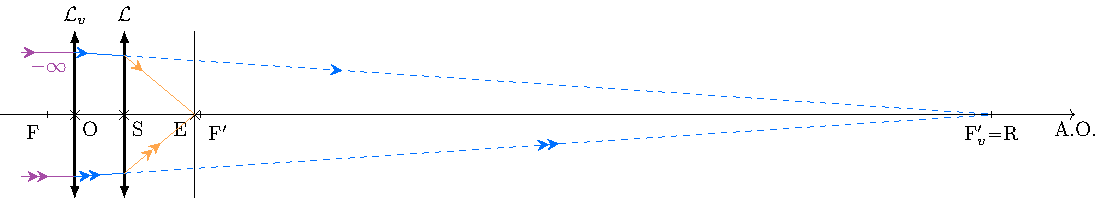
\includegraphics{ch3-3-3}
\end{center}

\section{Ordonnance d'un ophtalmologiste}
\begin{tcbraster}[raster columns=3, raster equal height=rows]
    \begin{NCdefi}{Définitions}
        L'ophtalmologiste donne une prescription pour fabriquer des verres
        correcteurs. Les valeurs correspondent donc aux caractéristiques et
        verres nécessaires à la correction.
    \end{NCdefi}
    \begin{NCdemo}{Outil}
        $f' = 1/V$, et pour une lentille convergente $f' > 0$.
    \end{NCdemo}
    \begin{NCexem}{Application}
        Les verres correcteurs sont donc divergents. On en conclue que M. Dupont
        a des yeux trop convergents, et qu'il est donc myope.
    \end{NCexem}
\end{tcbraster}

\section{Image à travers un doublet de lentilles}
\begin{tcbraster}[raster columns=3, raster equal height=rows]
    \begin{NCdefi}{Données}
        \begin{itemize}
            \item $(\Lc_1, O_1, f_1'= \SI{2.0}{cm})$ ;
            \item $\obar{O_1O_2} = \SI{+6.0}{cm}$ ;
            \item $(\Lc_2, O_2, f_2' = \SI{2.0}{cm})$ ;
            \item $(AB) = \SI{1}{cm}$ ;
            \item $\obar{O_1A} = \SI{-6.0}{cm}$
        \end{itemize}
    \end{NCdefi}
    \begin{NCdemo}{Outils}
        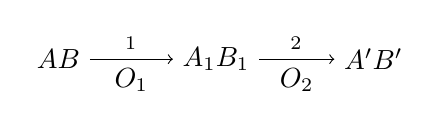
\begin{tikzpicture}[]
            \node[] (AB) at (0,0) {$\obar{AB}$};
            \node[] (A_1B_1) at (2,0) {$\obar{A_1B_1}$};
            \node[] (A'B') at (4,0) {$\obar{A'B'}$};
            \draw[->] (AB) -- (A_1B_1)
                node [midway, above] {$\Lc_1$}
                node [midway, below] {$O_1$};
            \draw[->] (A_1B_1) -- (A'B')
                node [midway, above] {$\Lc_2$}
                node [midway, below] {$O_2$};
            %\node[below=0.3, Purple!70] (ABb) at (AB) { \SI{-6}{cm}};
        \end{tikzpicture}
        \[\boxed{ \frac{1}{\OF} = \frac{1}{\OAp} - \frac{1}{\OA}}\]
        \[\gamma = \frac{\ABp}{\ABb} = \frac{\OAp}{\OA}\]
        \[\gamma_{\rm combinaison} = \gamma_1\times\gamma_2\]
    \end{NCdemo}
    \begin{NCexem}{Application}
        $\obar{O_1A_1} = \SI{3}{cm}$, $\obar{O_2A_1} = \SI{-3}{cm}$ donc
        \fbox{$\obar{O_2A'} = \SI{6}{cm}$} ;\smallbreak
        $\DS \gamma_{\rm doublet} = \frac{\ABp}{\ABb} =
        \frac{\obar{O_1A_1}}{\obar{O_1A}}\times
        \frac{\obar{O_2A'}}{\obar{O_2A_1}} = +1$ donc\smallbreak
        \fbox{$(\ABp) = (\ABb)$}
    \end{NCexem}
\end{tcbraster}
\begin{center}
    \begin{NCrema}{Schéma}
        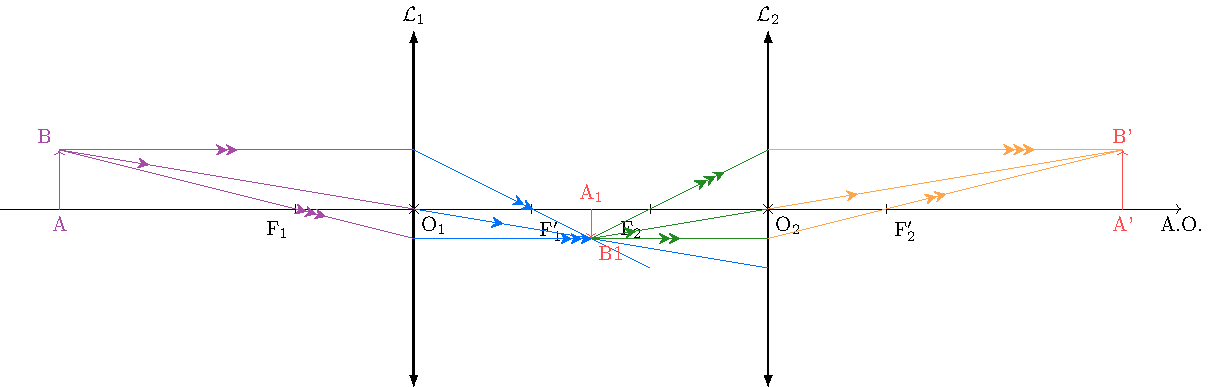
\includegraphics[width=\linewidth]{ch3-5}
    \end{NCrema}
\end{center}

\section{Une lunette astronomique}
Non traité.

\section{Les défauts de l'œil}
\begin{center}
    \begin{NCdefi}[width=.5\linewidth]{Donnée générale}
        
    \end{NCdefi}
\end{center}
\subsection{Œil myope}
\begin{tcbraster}[raster columns=2, raster equal height=rows]
    \begin{NCdefi}{Données}
        Avec les données sur le champ de vision :
        \begin{itemize}
            \item $\obar{SR} = \SI{-1}{m}$
            \item $\obar{SP} = \SI{-30}{cm}$
        \end{itemize}
        De plus, on a $(\Lc_v, O_v, V_v = \SI{-1}{\de})$.
    \end{NCdefi}
    \begin{NCdemo}{Outil}
        Pour l'œil au repos :
        \begin{tikzpicture}[]
            \node[] (AB) at (0,0) {$\obar{AB}$};
            \node[] (A_1B_1) at (2,0) {$\obar{A_1B_1}$};
            \node[] (A'B') at (4,0) {$\obar{A'B'}$};
            \draw[->] (AB) -- (A_1B_1)
                node [midway, above] {$\Lc_v$}
                node [midway, below] {$O_v$};
            \draw[->] (A_1B_1) -- (A'B')
                node [midway, above] {$\Lc$}
                node [midway, below] {$S$};
            \node[below=0.3, Purple!70] (ABb) at (AB) {$?$};
            \node[below=0.3, brandeisblue] (A_1B_1b) at (A_1B_1) {$A_1 = R$};
            \node[below=0.3, orange!70] (A'B'b) at (A'B') {$A' = E$};
            \draw[->, Purple!70] (ABb) to[bend right] (A_1B_1b.west);
            \draw[->, orange!70] (A'B'b) to[bend left] (A_1B_1b.east);
        \end{tikzpicture}
    \end{NCdemo}
\end{tcbraster}

\theendnotes
\end{document}
